\begin{titlepage}
    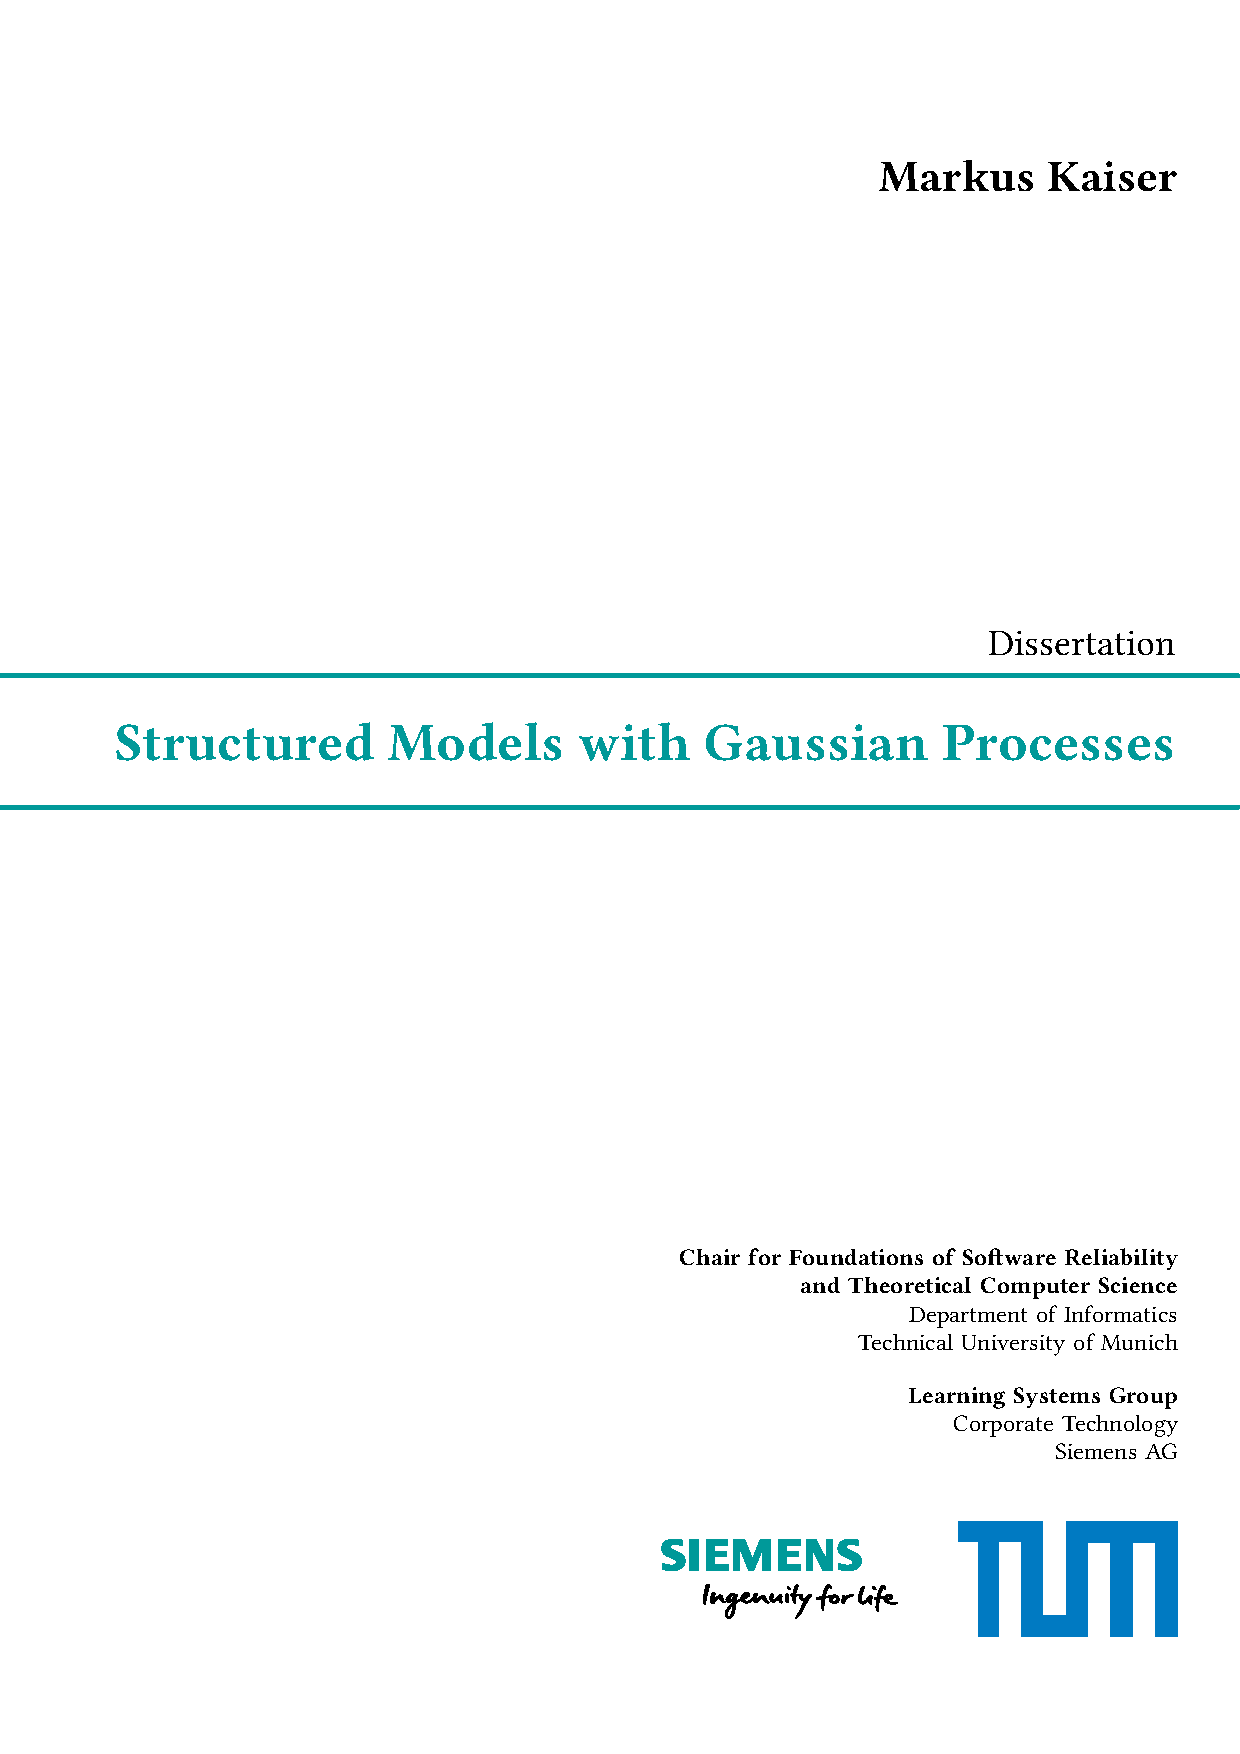
\includepdf{figures/title_page}
\end{titlepage}

\begin{titlepage}
    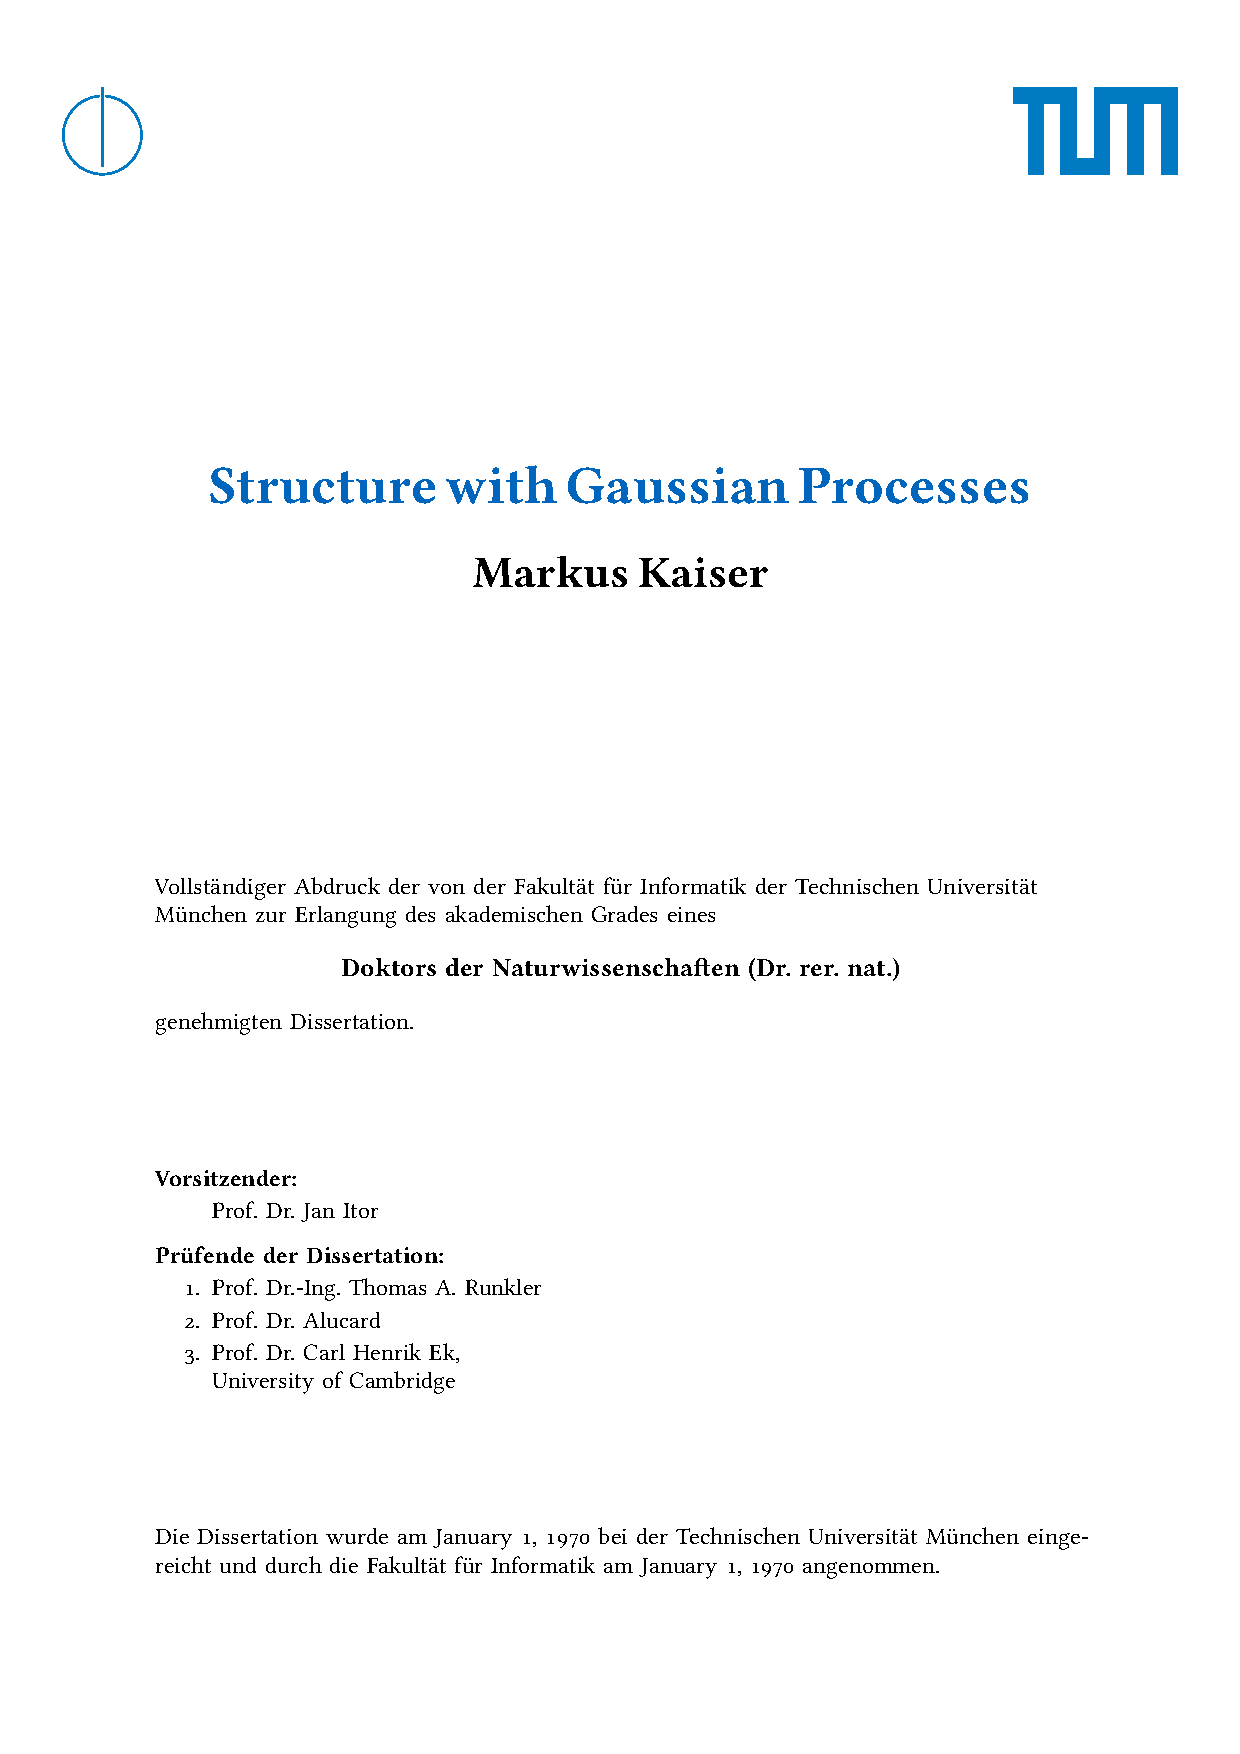
\includepdf{figures/title_page_tum}
\end{titlepage}

\begin{Abstract}{ngerman}
    \todoi{German abstract}
\end{Abstract}

\begin{Abstract}{english}
    Machine learning methods have seen great success recently in a wide range of digital domains such as speech recognition, computer vision or video games.
    However, bridging the gap to applications in the physical world has proved challenging as they introduce a new set of requirements.
    Machine learning systems must make efficient use of expert knowledge, handle low data regimes, and quantify uncertainties.
    This thesis studies how structured probabilistic models allow us to cope with these requirements.
    Structured models combine black-box and white-box modeling approaches to formalize expert knowledge while still being able to gain new insights from data.
    While in white-box models experts design components to describe a generative process in great detail, black-box models rely on general function approximators and trust that structure can be extracted given enough data.
    In structured models, we make use of available expert knowledge but accept that there are parts of the system we do not understand and model them using black-box components.
    Imposing structure allows us to characterize desired solutions and formulate what we want to learn from data.

    In this work, we study how to formulate Bayesian structural models using methods from Bayesian nonparametrics.
    We interpret recent advances in inference schemes for deep Gaussian processes in the context of structural models and formulate informative hierarchical priors.
    We discuss two approaches to adding structure based on mathematical formalization and expert-understanding of an underlying physical process.
    Using real-world industrial applications such as the detection of faulty sensors and the prediction of power generation in a wind-farm as examples, we show how structural priors lead to models with rich internal structure and physically plausible results.

    In situations where internal structure or generalization behavior come into focus, model selection using marginal likelihoods can be insufficient to identify desirable models.
    We consider how to formalize the subjectiveness in model selection through the task a model will be used to solve.
    We show that in a reinforcement learning problem, semantic models outperform other models with similar performance metrics and allow experts to influence agent behavior.
    We finally discuss why models with suboptimal marginal likelihoods can perform well in hierarchical systems and consider how to formulate Bayesian inference problems that take downstream tasks into account.
\end{Abstract}

\begin{Acknowledgements}
    \todoi{Acknowledgements}

    \begin{itemize}
        \item Thomas Runkler, Carl Henrik Ek, Clemens Otte
        \item Volkmar Sterzing, Steffen Udluft, Daniel Hein, Stefan Depeweg, Philipp (?), (Marion, Christoph, Dieter), LSY
        \item Neill Campbell, Erik Bodin, Ieva Kazlauskaite, Ivan Ustyuzhaniov, Bristol and Bath
        \item Pia und Robert, Andrea und Matthias
        \item Hannah
    \end{itemize}
\end{Acknowledgements}

\listoftodos
\todototoc

\tableofcontents
